\newcommand{\DioptrikLetterFifteenDiagram}{%
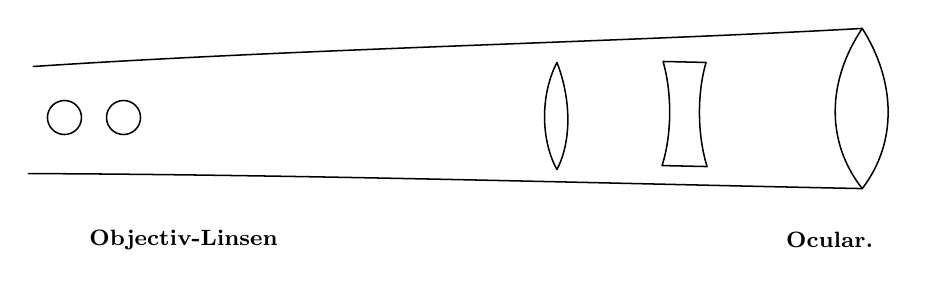
\begin{tikzpicture}[x=.005in,y=-.005in,line width=.55pt,line cap=round,line join=round]
\draw (42,71) .. controls (315,53) and (620,47) .. (870,33);
\draw (37,178) .. controls (315,179) and (620,188) .. (870,193);
\draw (870,33) .. controls (903,85) and (906,146) .. (870,193)
  .. controls (833,146) and (835,85) .. (870,33);
\draw (565,67) .. controls (578,100) and (581,143) .. (565,174)
  .. controls (549,145) and (548,100) .. (565,67);
\draw (671,66) -- (714,67) .. controls (705,97) and (705,139) .. (715,171)
  -- (670,170) .. controls (680,139) and (680,97) .. (671,66);
\draw (73,122) circle[radius=17];
\draw (132,122) circle[radius=17];
\node[anchor=west,font=\footnotesize\bfseries] at (88,244) {Objectiv-Linsen};
\node[anchor=west,font=\footnotesize\bfseries] at (784,244) {Ocular.};
\end{tikzpicture}%
}
